\documentclass[11pt]{report}

\usepackage[top=0.5in, bottom=0.5in, left=0.5in, right=0.5in]{geometry}
\usepackage{authblk}
\usepackage{hyperref}
\usepackage[utf8]{inputenc}
\usepackage{amsmath}
\usepackage{amsfonts}
\usepackage{amssymb}
\usepackage{siunitx}
\usepackage{graphicx}
\usepackage{subcaption}
\usepackage{float}
\usepackage[nottoc,numbib]{tocbibind}
\usepackage{biblatex}
\usepackage{parskip}
\usepackage{pdfpages}

\bibliography{references.bib}


\begin{document}
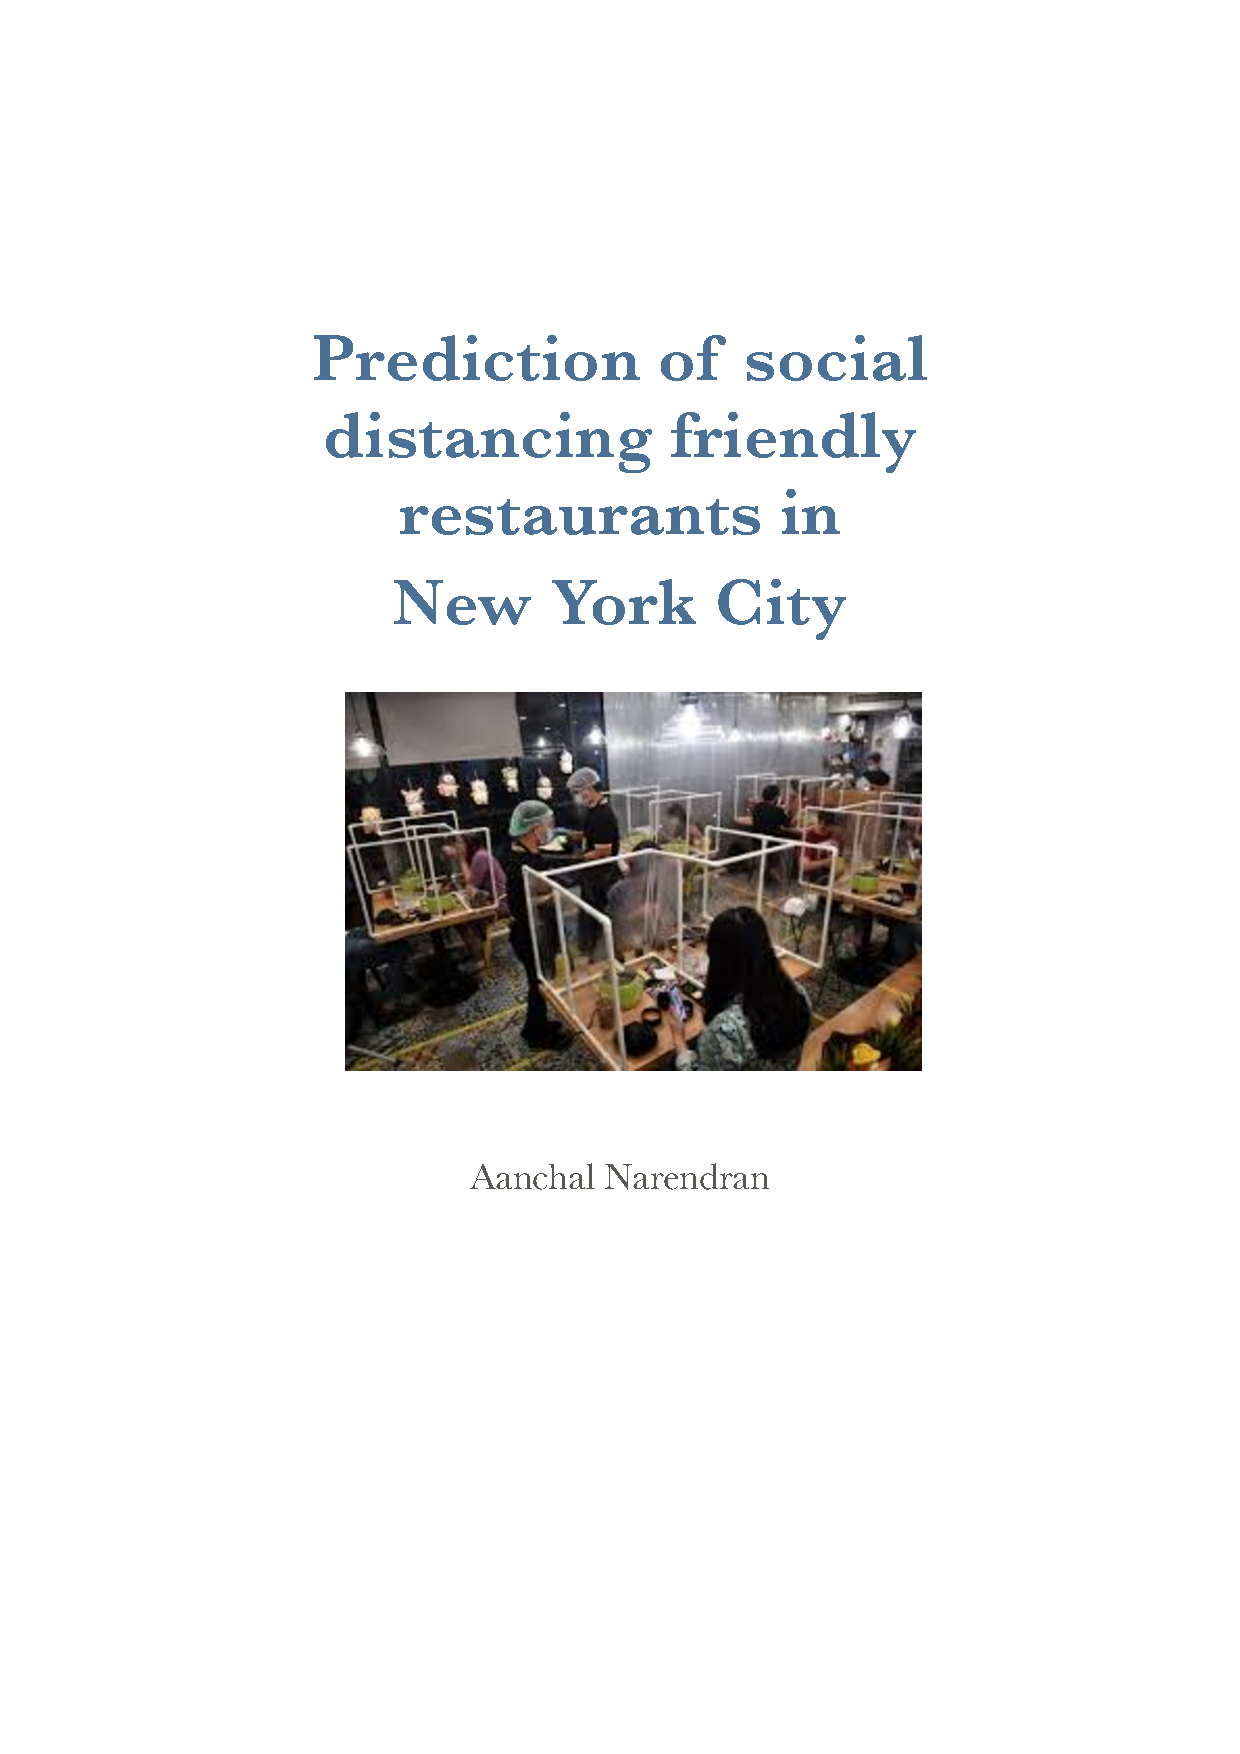
\includepdf[pages={1}]{corona_coverpage.pdf} 

\chapter{Introduction}

\par 
The restaurant business in New York City is unlike other business in the world. With 50,133 eating or drinking locations \cite{restaurants_statistics} and employing over 684,100 people \cite{restaurants_statistics} , The restaurant industry is vital to the economic and social fabric of New York City. Restaurants also aid in the development of local communities throughout the state.During the period of 2013-2016, approximately 37 percent of adults consumed fast food on a given day \cite{fastfood_percent:paper}.Studies have shown that consumption of food eaten away from home has also risen alarmingly. As of March 17, all restaurants in New York City have been banned from serving customers in house and many have completely closed doors. The spending in restaurants was down by 90 percent in late March, as opposed to the same time period last year \cite{NewYorkBudget:paper}. As New York City is entering the phase 3 of it's reopening, The number of employees at work place would be higher increasing the necessity for food being outsourced. 
\par The project aims to predict the most low risk restaurants in a certain neighborhood. This criteria has been determined by the center for disease control and prevention. It will prompt the user to input the neighborhood they are currently situated in based on which it would display the most low risk restaurants. The program devised can be used as a stand alone application or be integrated with existing restaurant  recommendation systems. It's user base is not limited to any sect, age or category of citizens.

\chapter{Data}
\par For this project, We will majorly be using 4 datasets/data sources. They are as follows:
\begin{enumerate}
    \item Foursquare places API: Extract names of restaurants and their details
    \item New York JSON: Contains all neighbourhood and boroughs as well as their coordinates
    \item Cases by Borough: Contains list of active number of cases in a borough
    \item Census New York City: Contains the list of boroughs as well as their area which will aid as a normalising factor
\end{enumerate}
\par The Foursquare API has a list of all the restaurants in the neighborhood. In this case we aim to use the venue endpoint. The venue api call takes the Latitude and Longitude, Limit, Radius and Category id as parameters. In the project's case, the limit is set to 35 owing to Foursquare's premium api calls quota. The Radius is limited to ensure the containment of a person to their borough. CategoryId is set to that of restaurants to ensure only extraction of food related spots. The user is prompted to input their neighbourhood which is used for extraction of Latitude and Longitude.The venue details endpoints returns a json with basic details of the venue. We extract the venue id, name, category, address and delivery provider. We extract a series of the venue id's to create a foursquare details api call which is a premium call. The details endpoint returns one json entry per id which contains rich data about the venue. We extract the Rating, Price point, Contact no, Menu, Parking, Seating and reservations data of the venue. According to CDC, Restaurants which have drivethroughs, delivery, take out and curb side pickup are low risk restaurants\cite{restaurantconsiderations:article}. Outside seating makes it a comparatively more risk restaurant. Inside seating is even more risk. 
\par The New York json file contains the list of the borough, neighbourhood and the generic coordinates of the neighbourhood. We extract this json to collect the coordinates for the foursquare api call. We also use it to generate a folium map to plot the neighbourhood and the restaurants obtained out of the filters. 
\par The active number of cases would work as a cutoff. In the end result, if the active number of cases is greater than a certain threshold value, It would prompt the user to stick to delivery options. We also extract the areas data inorder to ensure normalization. For instance Manhattan is populated with high rise buildings, This increases the population density. Hence we normalize it by using number of active cases divide by area. 

\chapter{Methodology}
\par The generic execution of the code starts with collecting the data from numerous source and reading them into dataframes. We then prompt the user for an input of the neighbourhood name and extract coordinates. These coordinates are used for the foursquare api calls and collect the restaurants data. This data is passed through filters and then graphed on a map using Folium. 
\par The first part of the code starts with using wget to collect the New York json file. We extract the neighbourhood, borough, latitude and longitude values which is then appended entry by entry to the neighborhoods dataframe. We then use pandas to read the boro.csv from nychealth's covid repository which contains the number of active cases per day in the borough. We then extract the area of the borough. We use it to normalize the number of cases in the borough. 
\par We prompt the user to input the neighbourhood they're currently located in. On locating the borough, Latitude and Longitude, we display them just for additional benefit. The latitude and Longitude hence extracted is then used to make the foursquare api call. We extract 35 locations in the vicinity of the neighbourhood. We extract the id, name, address, Category, Latitude and Longitude, and delivery provider of the venue. The id extracted aides us in the next part of the program. The latitude and longitude extracted is later on used to plot the restaurant on a map generated by folium. 
\par We use the id's of restaurants previously extracted to generate a listing of all details with regards to the venue. The json extracted consists of very rich data and we only extract the data relevant to either the user or to us. We extract the rating, phone number, price point, menu, seating type, parking and reservations details of the venue. The seating type, parking, reservation details and delivery option are used to generate the social distancing rating. For now the grading scale is out of 4. If the venue has outdoor seating, the venue gets a +1 else there is no change. The parking if street gives the rating a +1. The delivery option also gives the venue a +1. \cite{restaurantconsiderations:article} Although reservations are not mentioned by the Center of disease control and prevention, it logically makes sense as the reservations aspect can be used to control the number of people in a restaurant at any point of time. 
\par The data hence obtained is converted into a dataframe. We then extract the number of active cases in the borough as well as the area to normalise it. If it's greater than the cutoff constraint, We prompt the user to stick to delivery options and provide them with a list of the best restaurants around them and their delivery provider. If it's lesser than the constraint, We display those restaurants which meet any one or more of the considerations cited by the Center of disease control and prevention \cite{restaurantconsiderations:article}. We sort these recommendations on the basis of the social distancing friendly rating rather than the general rating. 
\par We now plot all of the locations obtained by the filter on a map generated by Folium. The red circle denoted the generic location of the neighbourhood. The dark green circle denotes the best option. The Light green circle denotes the second best option. The Orange circle denotes the third best option. The pink circles are used to denote the rest of the options. 
\par An accurate representation of the basic function of the code can be viewed with figure \ref{flowchart}

\begin{figure}[ht]
  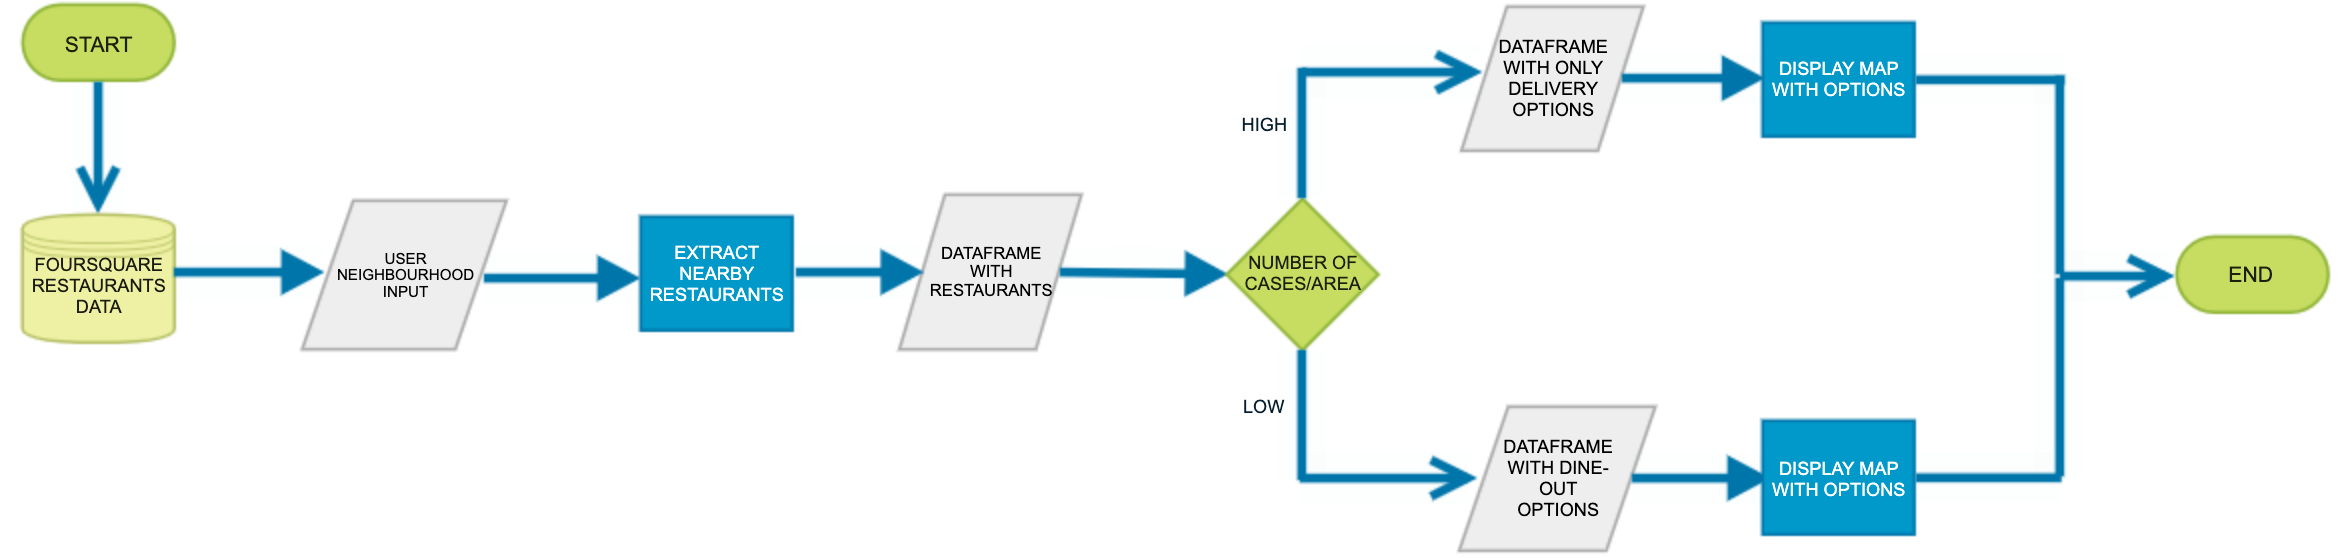
\includegraphics[width =\columnwidth]{flowchart.png}
  \caption{Flowchart of function}
  \label{flowchart}
\end{figure}

\chapter{Results}
\par The results of this project are purely qualitative and cannot be quantified. The results would be the output that the user recives in the form of a dataframe withe details of the restaurant as well as a folium map with all the markings explained in the methodology. 
\par The neighbourhood in question here is east village. The first two pictures represent the output as of date. The figure \ref{df_delivery} is a dataframe depicting all the options that a user has for delivery. This dataframe is just a part of the much longer dataframe. It has the name, delivery provider, contact no and price range of the restaurant. In this case sorting is done based on the actual rating of the restaurant as the social distancing rating doesn't hold much relevance in this case. The figure \ref{map_delivery} is the folium map that is generated based off of the dataframe in figure \ref{df_delivery}

\begin{figure}[ht]
  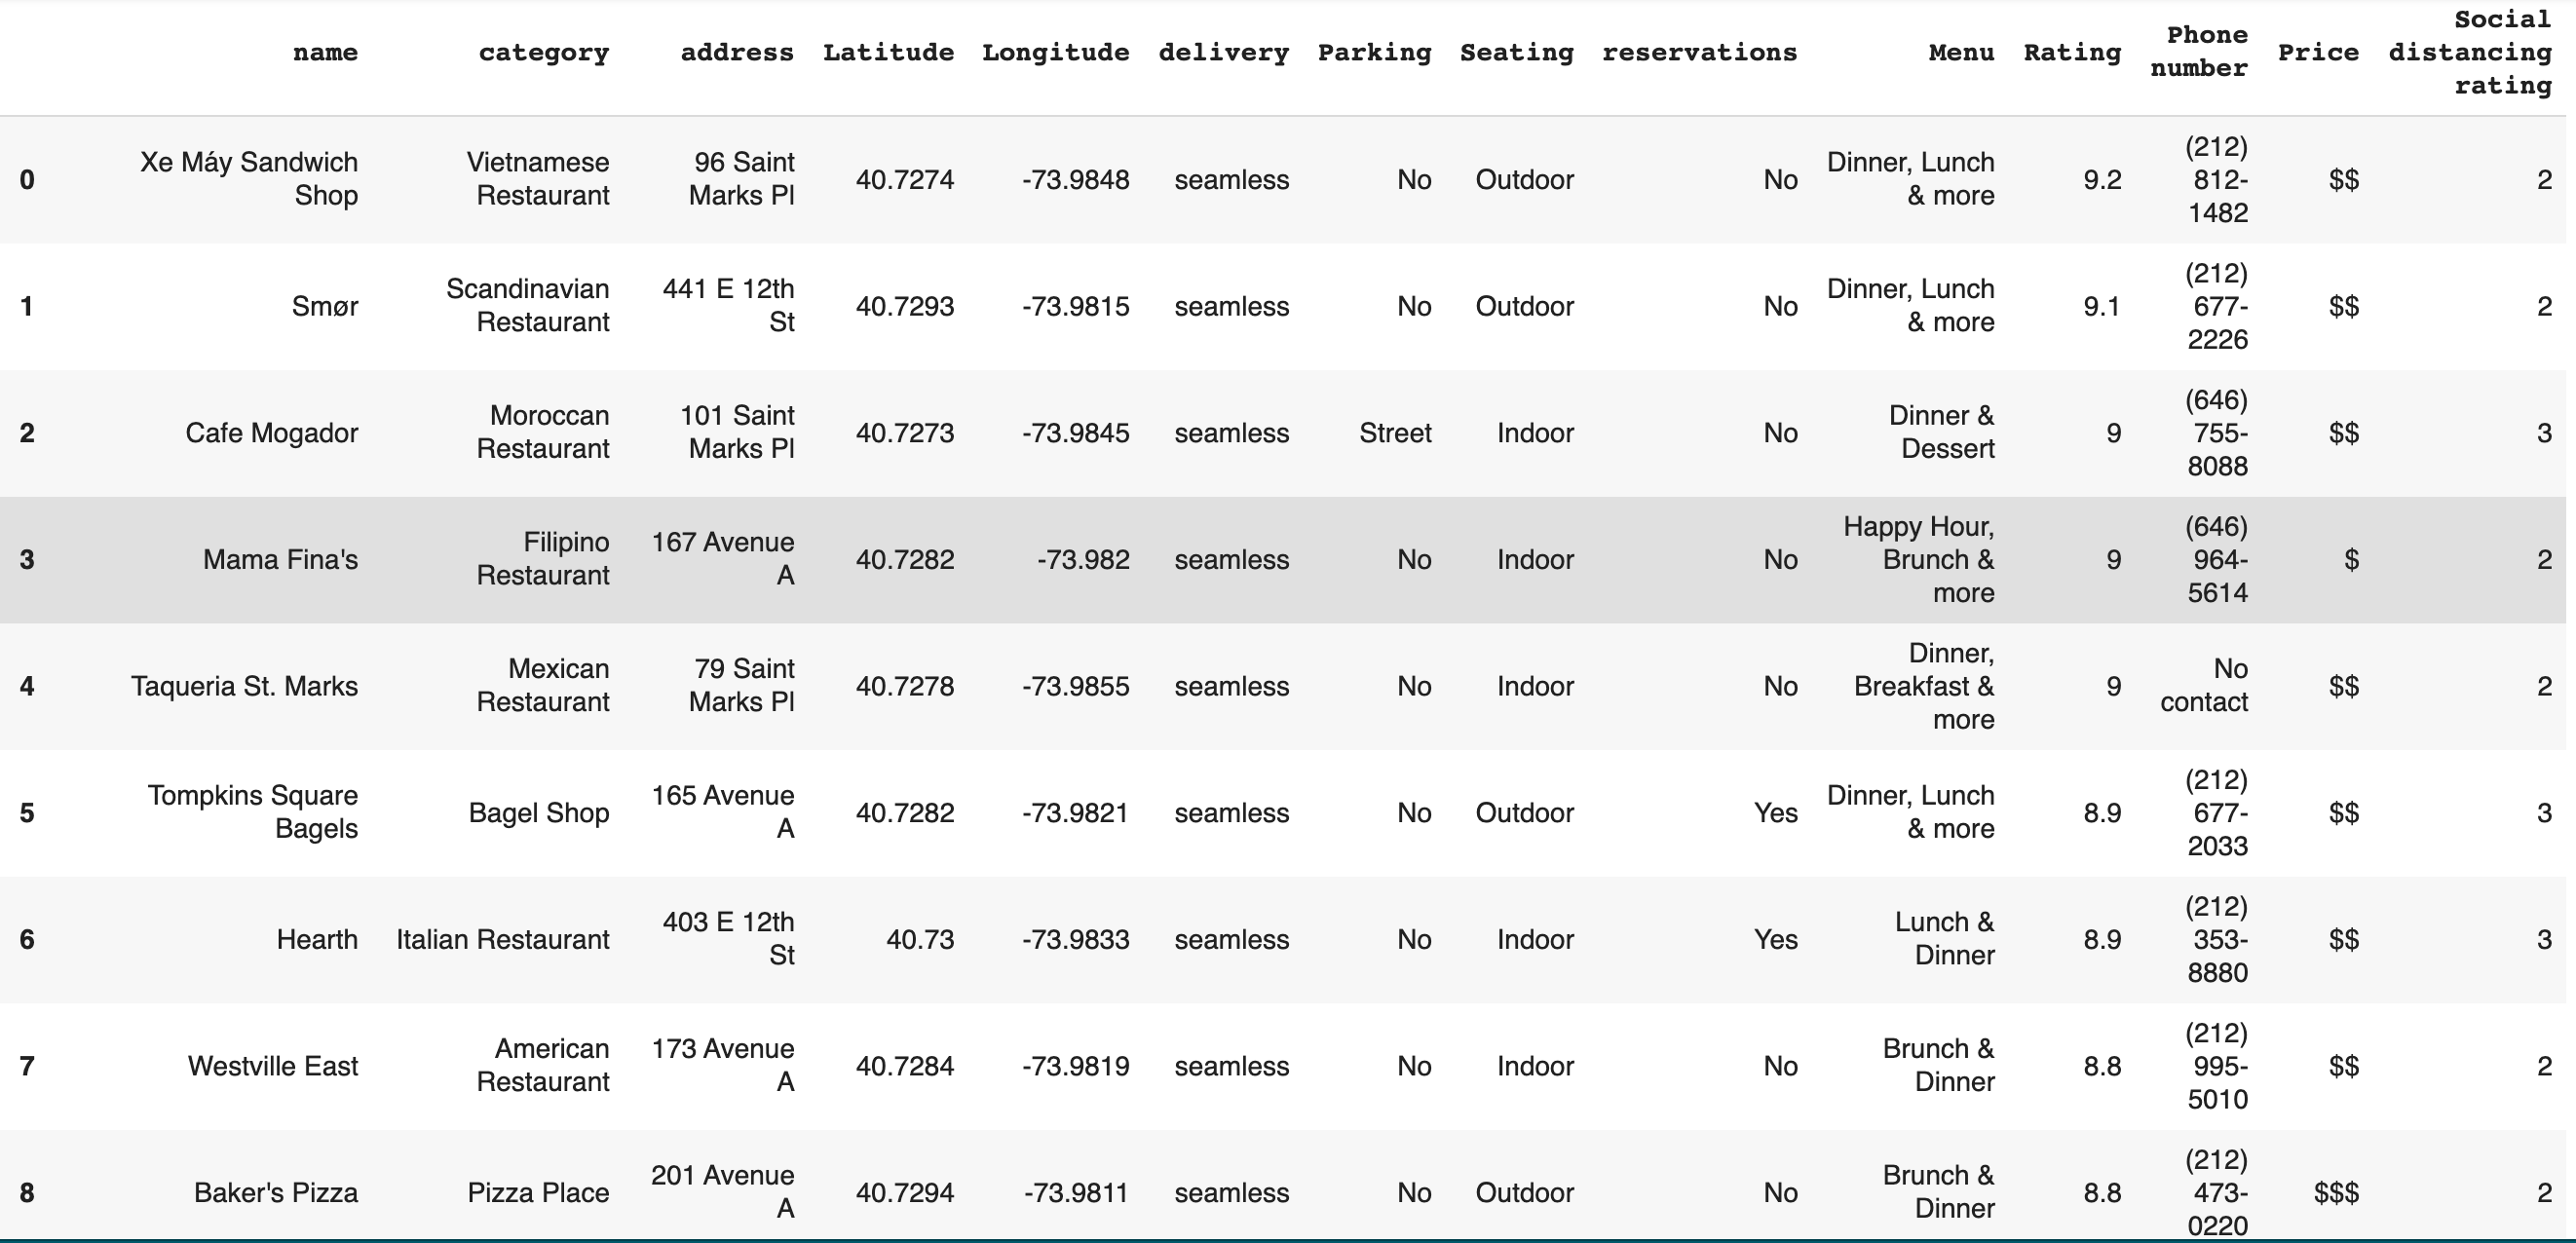
\includegraphics[width =\columnwidth]{east-village-delivery-data.png}
  \caption{Dataframe of delivery data}
  \label{df_delivery}
\end{figure}

\begin{figure}[ht]
  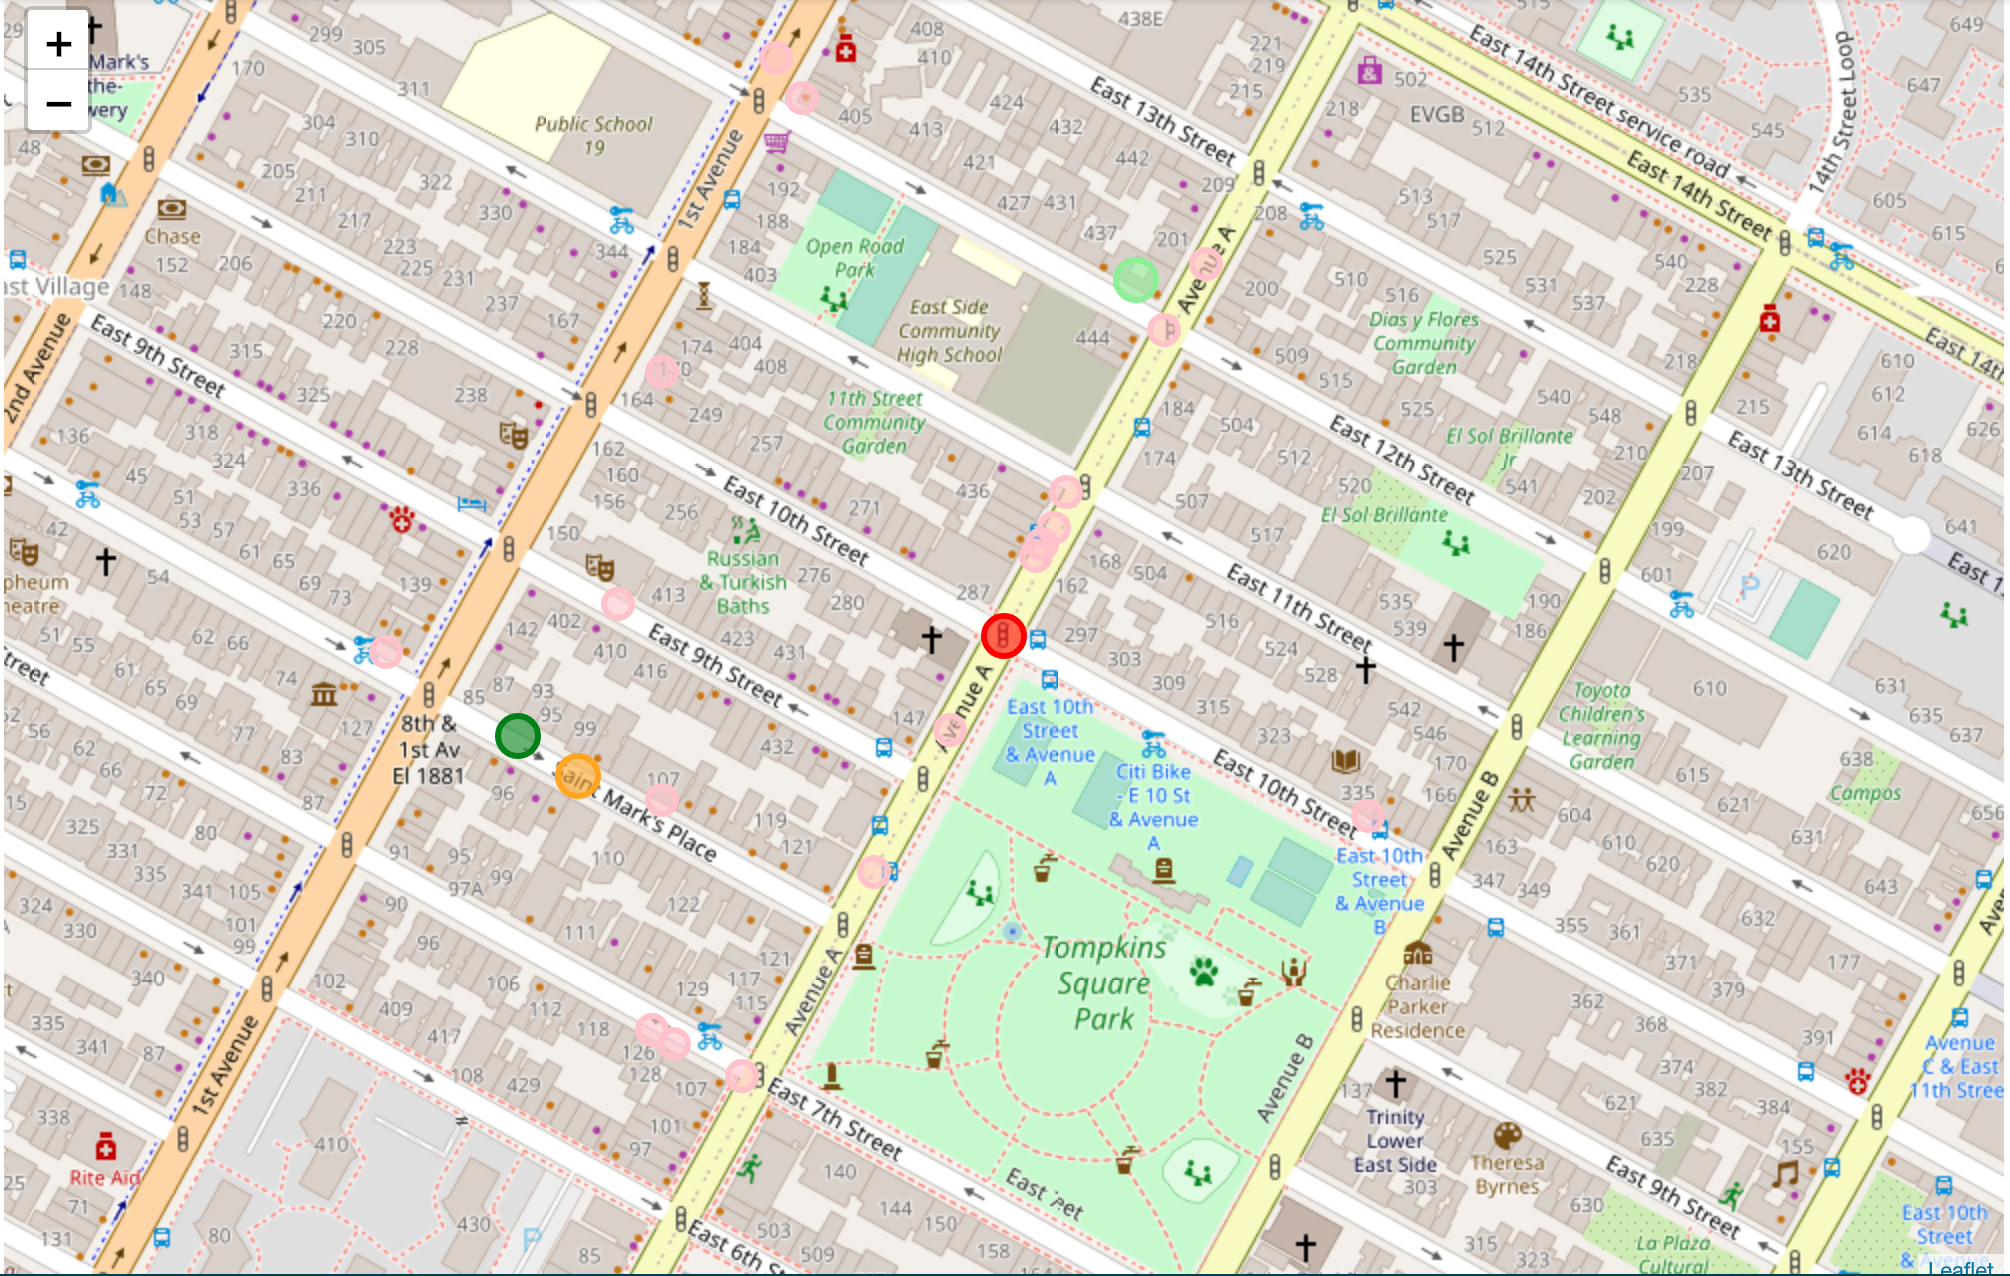
\includegraphics[width =\columnwidth]{east-village-delivery.png}
  \caption{Map of delivery restaurants}
  \label{map_delivery}
\end{figure}

\par This case is currently an hypothetical case after the coronavirus pandemic subsides. The figure \ref{df_dinein} depicts the dataframe with the name, address, contact number, parking options, seating options, reservation, price range and both the ratings. However unlike the previous case, the sorting here is done on basis of the social distancing rating. The figure \ref{map_dinein} shows the folium map based off of the data in figure \ref{df_dinein} 

\begin{figure}[ht]
  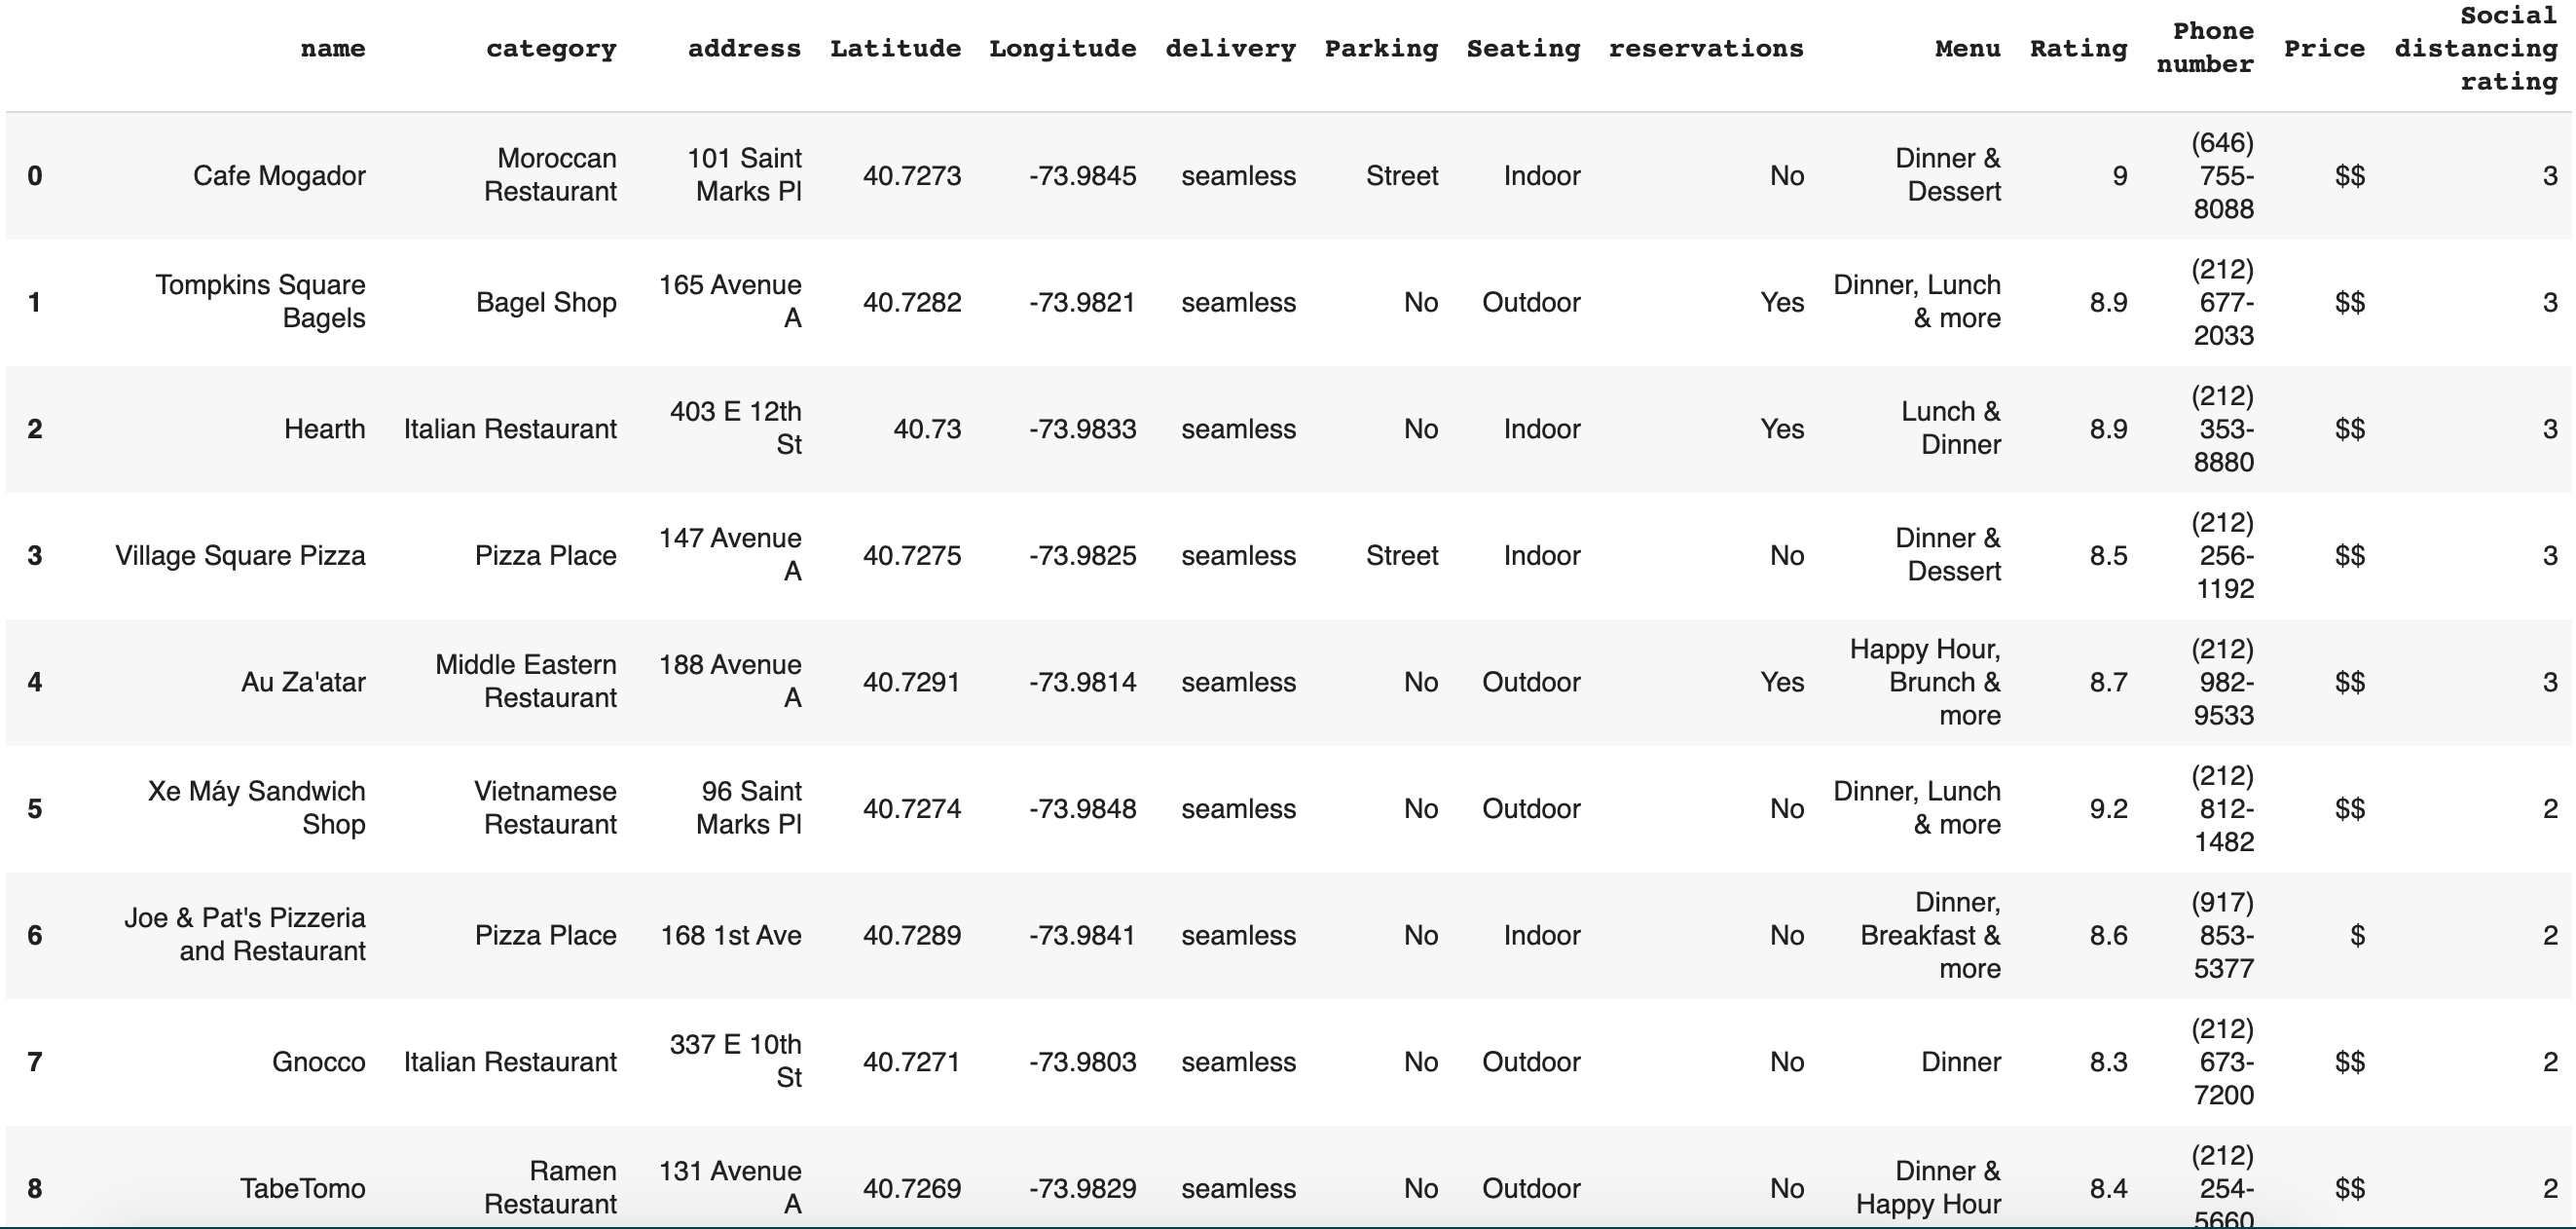
\includegraphics[width =\columnwidth]{east-village-dinein-data.png}
  \caption{Dataframe of dine in data}
  \label{df_dinein}
\end{figure}

\begin{figure}[ht]
  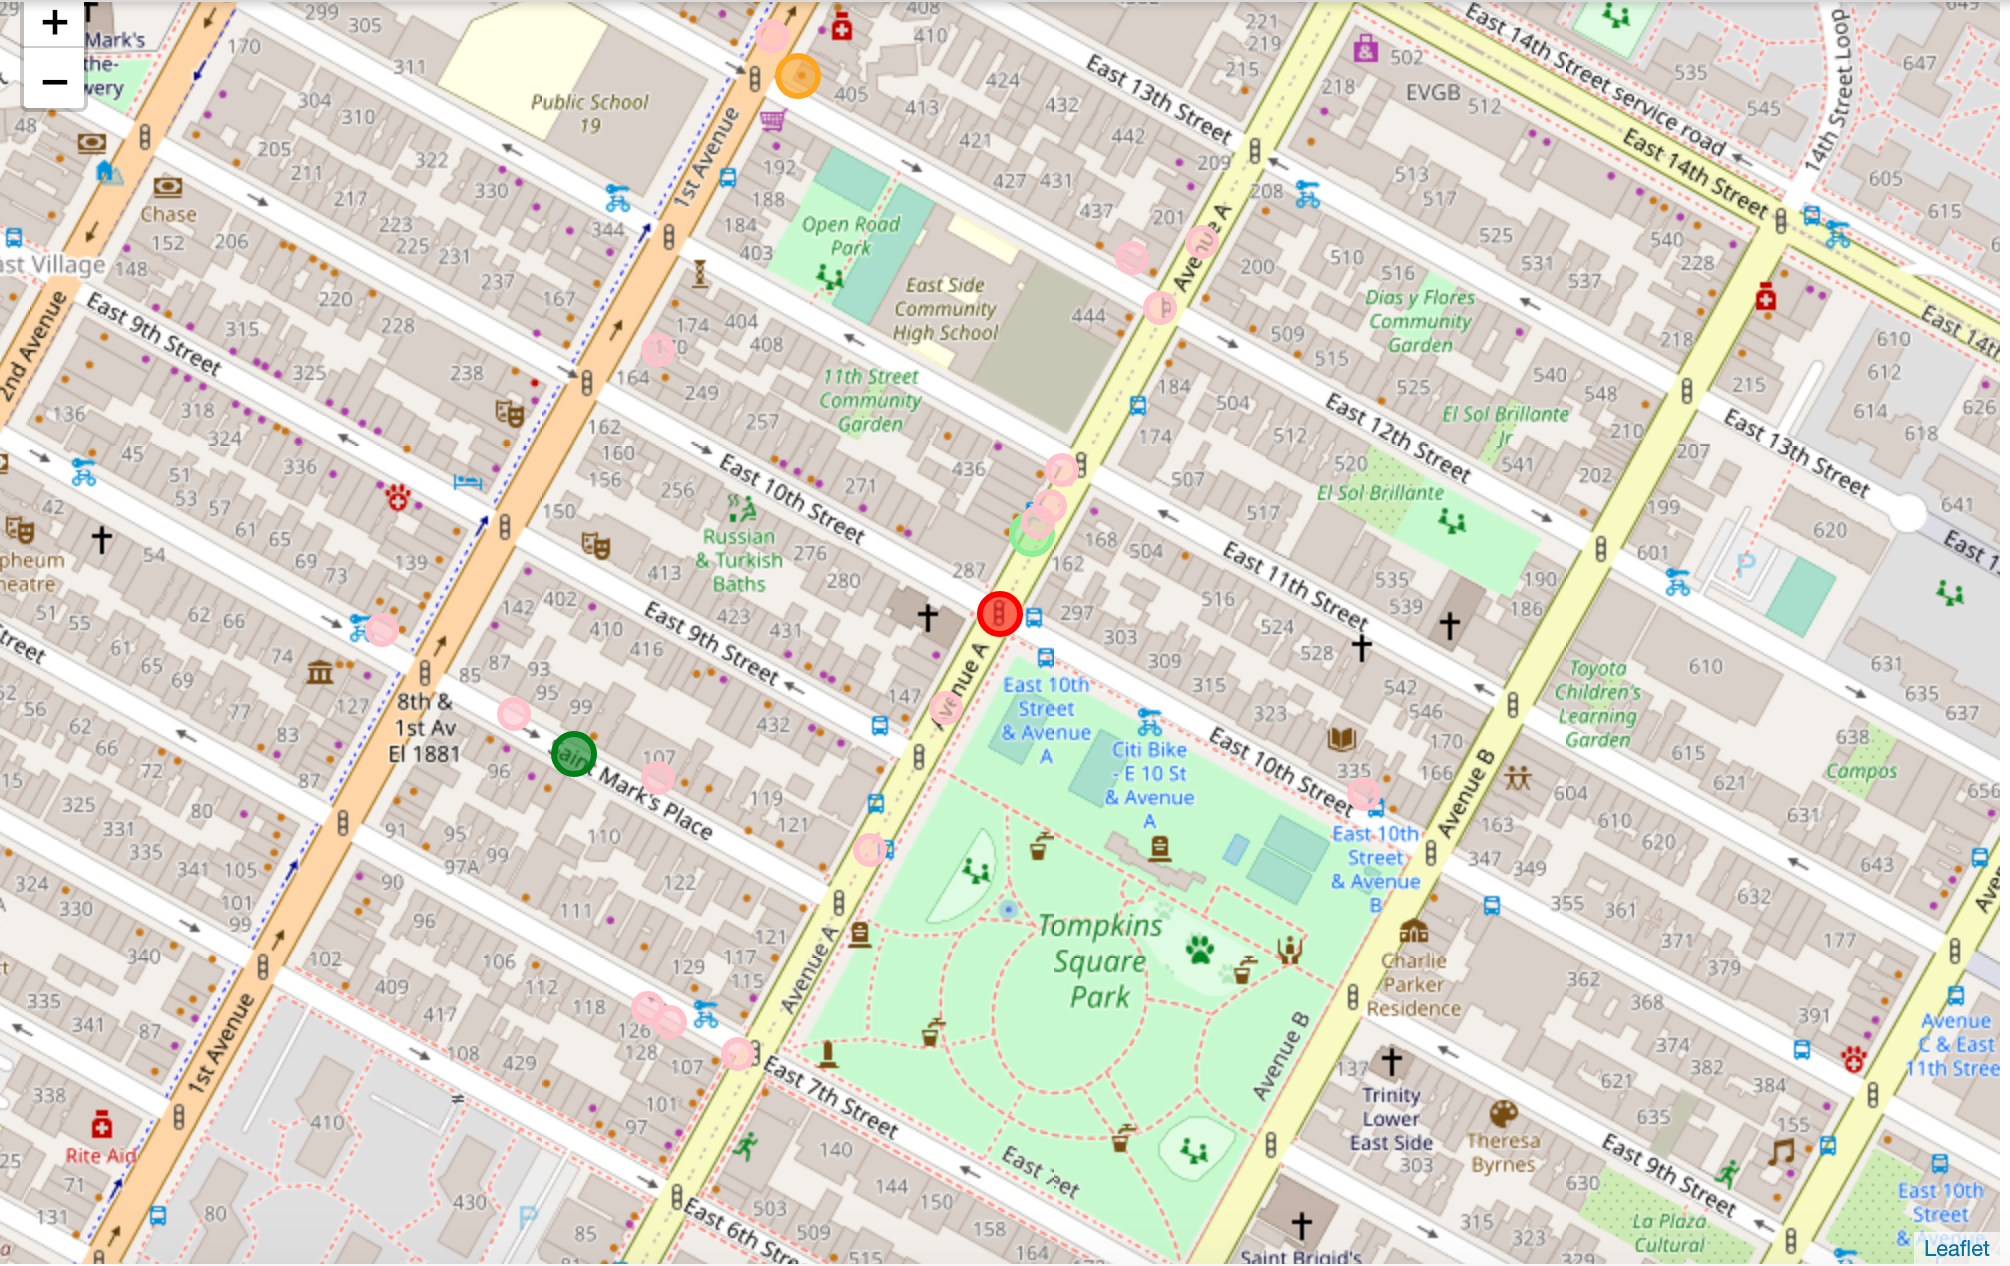
\includegraphics[width =\columnwidth]{east-village-dinein-map.png}
  \caption{Map of dine in restaurants}
  \label{map_dinein}
\end{figure}

\chapter{Discussion}
\par It's quiet evident from the data that a considerable chunk of restaurants which can be categorized as social distancing friendly also have a good rating overall. At the same time we must take into consideration that a good rating does not imply a good social distancing rating. This is owing to the fact that a vast majority of restaurants with higher rating are often indoor dining restaurants and have valet parking which increases the chances of primary contact. 
\par A decent amount of, if not all, restaurants have delivery ties. This is owing to the fact that New York City is not only home to a large number of universities but is also one of the world's financial centers. The universities imply a large chunk of millennial's and generation Z students who are more likely to stay indoors as opposed to the older generations. Being a financial district with long exhaustive hours, It's more than plausible that one would fall back to delivery options. 

\chapter{Conclusion}
\par We would conclude by stating that all said and done, This system is not as accurate as one would expect it to be. The future scope of this project would be integrate it with foursquare's pilgrim sdk to obtain real time location instead of solely relying on the user. These are truly trying times and this is just one of the many solutions out there that aims towards making the pandemic one step easier to tolerate and get through. 

\printbibliography
\end{document}